\begin{figure}[!htbp]
\centering
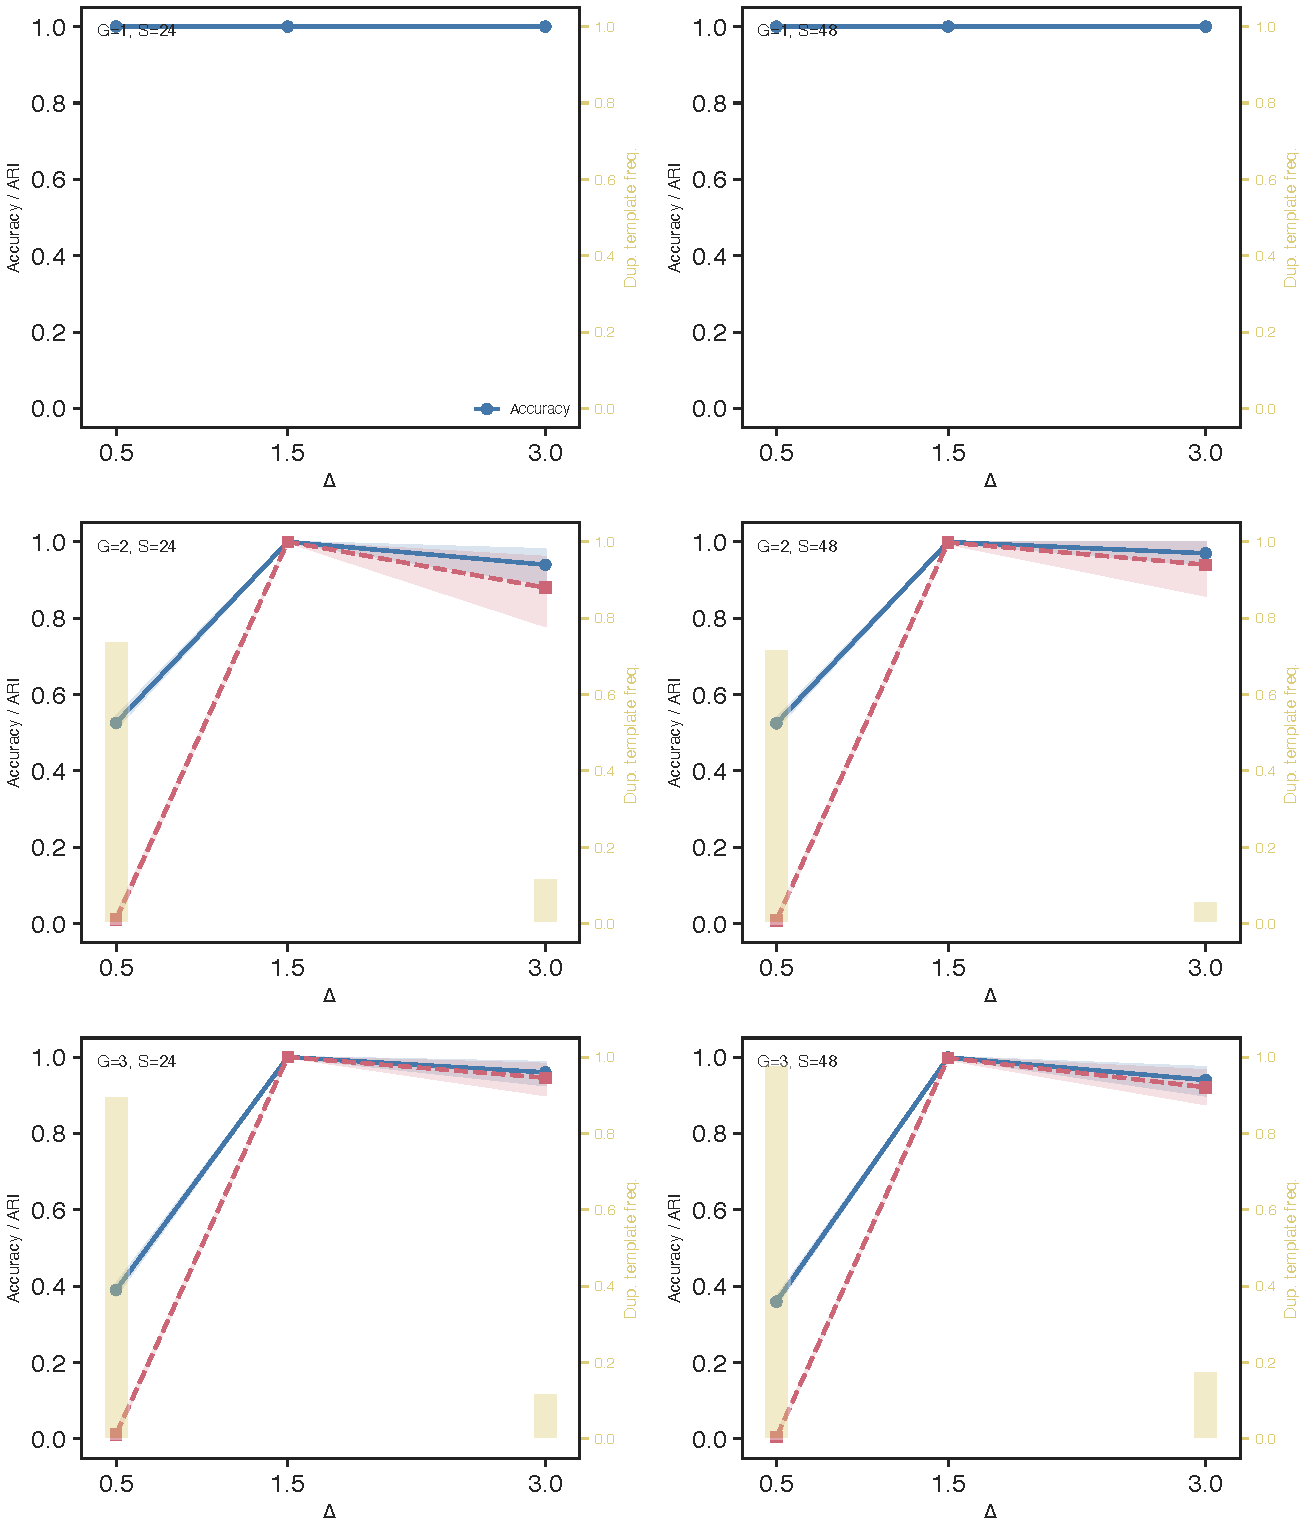
\includegraphics[width=0.96\linewidth]{shared/figures/results/fig_E05_templates.pdf}
\caption{E05 finite latent-template score clustering: label-permutation-invariant
hard accuracy (solid) and adjusted Rand index (dashed) vs signal separation $\Delta$,
with 95\% bootstrap bands. Bars show duplicate-template frequency (right axis).
Rows: $G\in\{1,2,3\}$ groups; columns: $S\in\{24,48\}$ sequences per dataset.
At $\Delta=0.5$, group templates collapse for $G\geq2$ and accuracy falls to
near-chance levels. At $\Delta=1.5$, accuracy and ARI approach 1.0.
At $\Delta=3.0$, mean accuracy is $0.940$--$0.970$ for $G=2$ and $0.940$--$0.960$
for $G=3$; duplicate templates appear in $6$--$18$\% of replicates, reflecting
local-optima sensitivity at strong signal.
For $G=1$ ARI is undefined and accuracy is 1.0 by construction.
All 900 objective traces are non-decreasing; no replicate failed.}
\label{fig:planned-templates-paper}
\end{figure}
